\documentclass[11pt]{article}
\usepackage{cse103}
\def\title{HW 4}

% use the tikz package to draw automata
\usepackage{tikz}
\usetikzlibrary{arrows,positioning,automata}

\begin{document}
\maketitle

\section*{Due October 27 at 11:59pm}

\textbf{(6 questions, 220 points total)}

\begin{qunlist}

\q{40}{Converting a DFA to a regular expression}\\
Convert the following DFA over the alphabet $\Sigma = \{x,y,z\}$ to a regular expression, showing the sequence of GNFAs you get along the way:

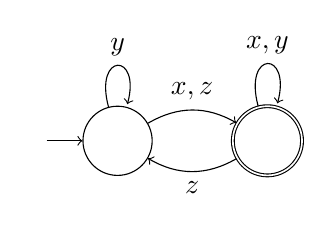
\begin{tikzpicture}
\node[state, initial, initial text=] (s1) {};
\node[state, accepting, right= of s1] (s2) {};

\path[->]
  (s1) edge[loop above] node[above] {$y$} (s1)
  (s1) edge[bend left] node[above] {$x, z$} (s2)
  (s2) edge[loop above] node[above] {$x,y$} (s2)
  (s2) edge[bend left] node[below] {$z$} (s1);
\end{tikzpicture}

\newpage

\q{50}{Proving non-regularity using the pumping lemma}\\
Use the pumping lemma to prove the following languages are not regular:

\begin{qparts}
\item
The language $L$ of correctly-nested parentheses (e.g. $(()()) \in L$ but $(() \not \in L$).

\item
The language $L = \{ x x^R \st x \in \Sigma^*\}$ over $\Sigma = \{0, 1\}$, where $x^R$ denotes the reversal of $x$ (e.g. $(100)^R = 001$).
\end{qparts}

\newpage

\q{30}{Big or small, not in-between}\\
Suppose that a regular language $L$ over $\Sigma$ is recognized by a DFA with $n$ states.
Prove that if $L$ is finite, then $|L| \le |\Sigma^{\le n-1}|$.
(So that if the language of a DFA is finite, it's at most exponentially-large in the number of states: regular languages are either infinite or at most exponentially-large.)

(\emph{Hint:} think about how we proved the pumping lemma.)

\newpage

\q{30}{Working with a CFG}\\
Consider the CFG $G$ with terminal symbols $\Sigma = \{ a, b, c \}$, nonterminal symbols $V = \{ S, T, U \}$, start symbol $S$, and the rules
\begin{align*}
S &\rightarrow aS \st Sb \st T \\
T &\rightarrow TT \st UU \\
U & \rightarrow c .
\end{align*}
For each of the following strings, state whether it can be derived from $G$, giving a derivation (a sequence of strings leading to it according to the rules) if so.

\begin{qparts}
\item $\epsilon$

\item $c$

\item $aaccccb$

\item $ab$

\item $abcc$

\item $cccccc$
\end{qparts}

\newpage 

\q{40}{Designing CFGs}\\
Give CFGs for the following languages:

\begin{qparts}
\item
With $\Sigma = \{ x, y, z, +, = \}$, let $L$ consist of all equalities between two sums of the variables $x, y, z$ with an equal number of terms on both sides.
For example the strings $x=x$ and $y+y=x+z$ are in $L$, but $x=y=z$ and $x=x+x$ are not.

\item
Suppose $x$ and $y$ are variables and $f(\cdot)$ and $g(\cdot, \cdot)$ are functions of 1 and 2 arguments respectively.
With $\Sigma = \{ f, g, x, y, (, ), \textbf{,} \}$ (where the last symbol is a comma), let $L$ consist of all valid expressions that can be built from these symbols without having triply-nested calls to $f$ (we don't restrict the depth of calls to $g$).
For example, the strings $x$, $f(f(y))$, and $g(x, g(f(x), f(y)))$ are in $L$, but $g(x)$ and $f(f(g(x, f(f(y)))))$ are not (the last example having 4 layers of calls to $f$).

(\emph{Hint:} First think about how to write the grammar without the nesting limit. Then you can elaborate your grammar to keep track of how many calls to $f$ you've already made.)
\end{qparts}

\newpage

\q{30}{Ambiguity}\\
For each of the following CFGs with $\Sigma = \{a,b\}$ and $V = \{S, T\}$, state whether it is ambiguous or unambiguous.
If it is ambiguous, give an example of two different leftmost derivations for a string.

\begin{qparts}
\item
\begin{flalign*}
S &\rightarrow TT \mid a &&\\
T &\rightarrow a \mid b &&
\end{flalign*}

\item
\begin{flalign*}
S &\rightarrow ST \mid Sb &&\\
T &\rightarrow a \mid b &&
\end{flalign*}

\item
\begin{flalign*}
S &\rightarrow TT \mid \varepsilon &&\\
T &\rightarrow TT \mid a \mid b &&
\end{flalign*}

\end{qparts}

\end{qunlist}
\end{document}